\documentclass[12pt]{article}
\usepackage[a4paper,height=23cm]{geometry}
\usepackage[tableposition=top]{caption}
\captionsetup{font=small,labelfont=bf,labelsep=period,singlelinecheck=false,
  width=13cm}
\usepackage{color}
\usepackage{graphicx}
\usepackage{parskip}
\usepackage[hidelinks,linktoc=all,pdfpagemode=None]{hyperref}
\definecolor{darkblue}{rgb}{0.0,0.2,0.6}
\definecolor{darkgray}{rgb}{0.2,0.2,0.2}
\newcommand\blue[1]{\textcolor{darkblue}{#1}}
\newcommand\gray[1]{\textcolor{darkgray}{#1}}
\newcommand\I[1]{\rule{0pt}{#1}}
\newcommand\gt{\raisebox{0.1ex}\textgreater}
\newcommand\SOFIA{{\sf SOFIA}}
\newcommand\sofialink[2]{\blue{\href{https://github.com/sofia-taf/#1}{\sf #2}}}
\frenchspacing
\setlength\hyphenpenalty{1000}
\hyphenation{calcu-lating reflect design develop-ment opposed experts control
  relevant}
\begin{document}

\thispagestyle{empty}

\begin{center}
  ~\\[0ex]
  \Large\bfseries SOFIA Transparent\\
  Analytical Framework\\[1.5ex]
  \large{\rm Design and development progress}\\[2.6cm]
  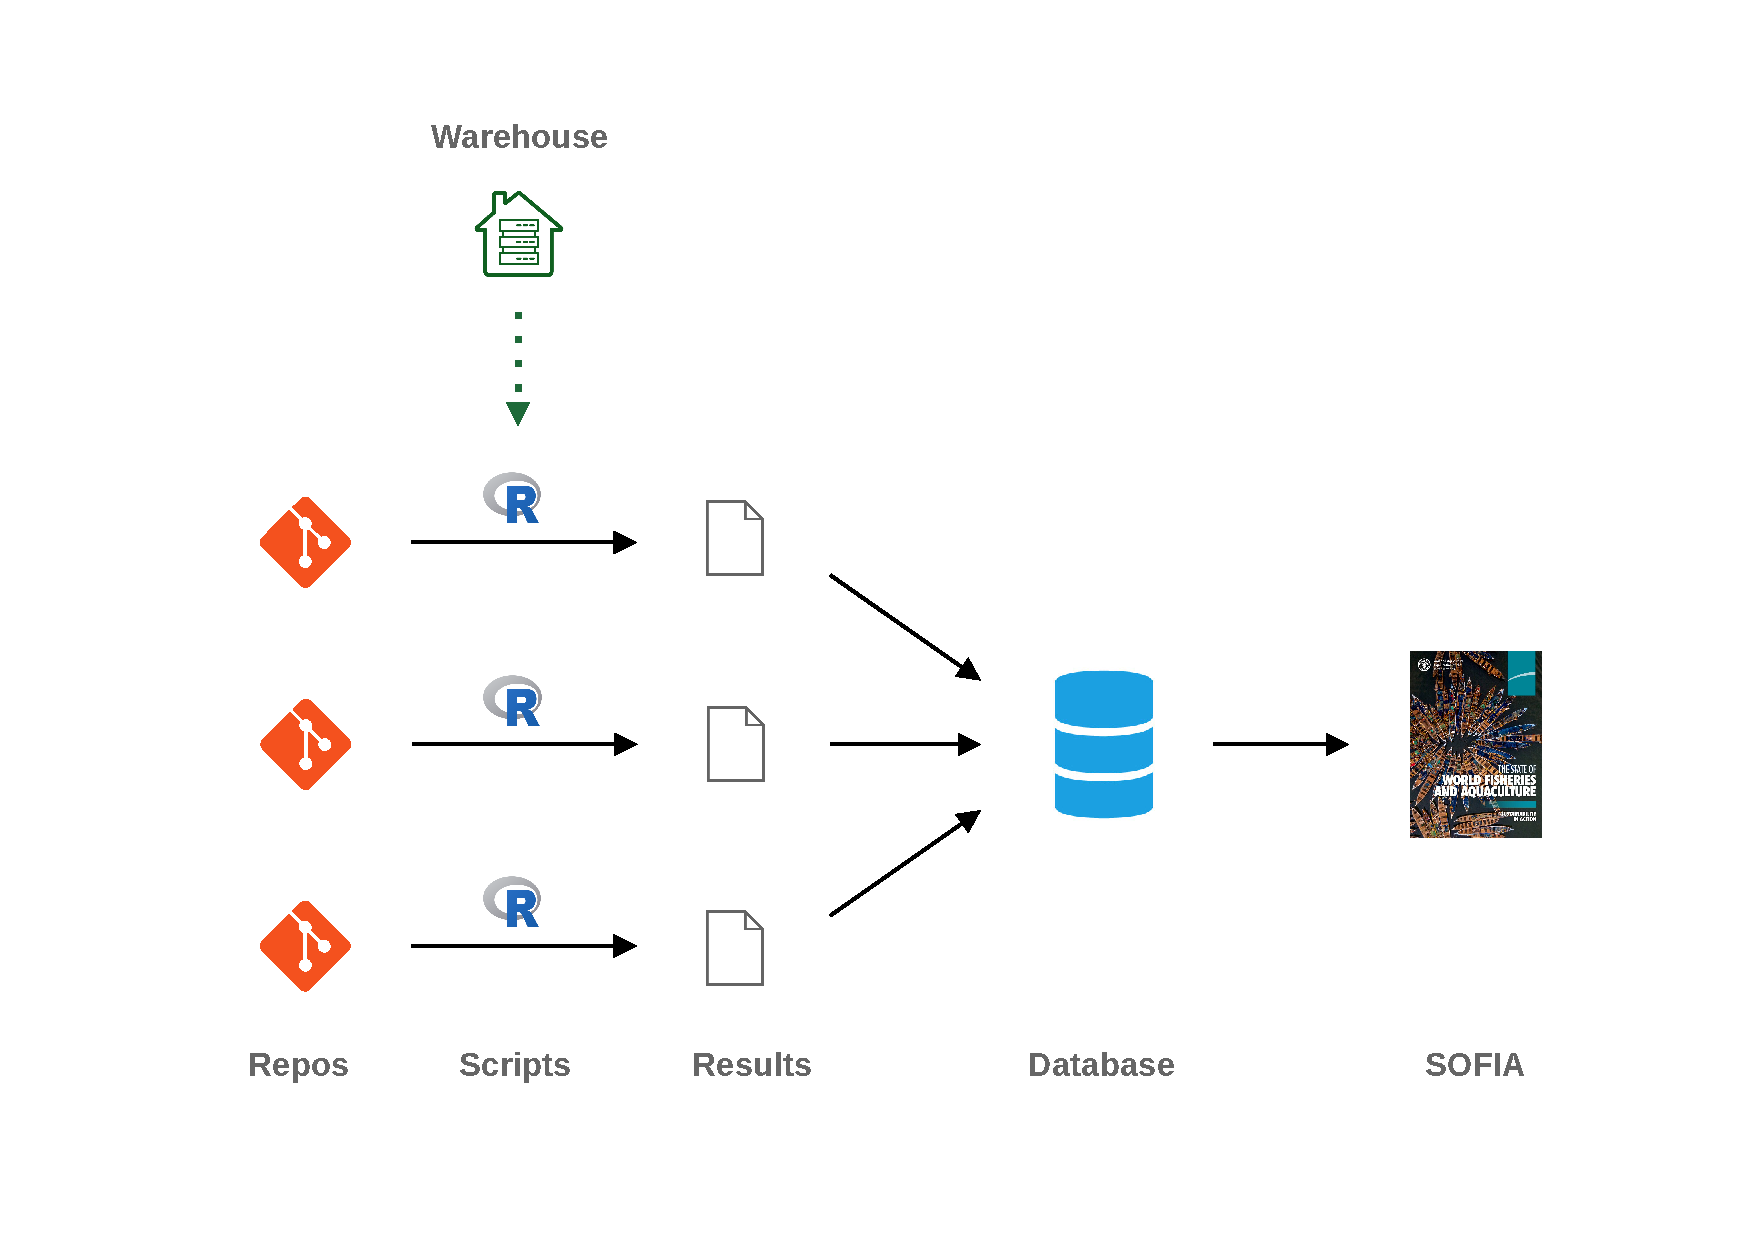
\includegraphics[width=0.64\textwidth]{sofia_taf_diagram}\\[1.5cm]
  \hspace{-1.5ex}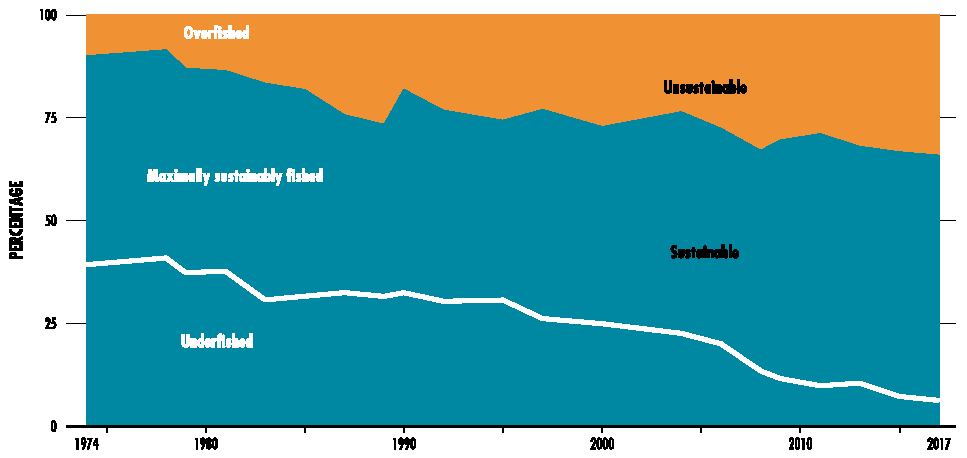
\includegraphics[width=0.75\textwidth]{sofia_fig19}\\[1.8cm]
  \mdseries Arni Magnusson\\[1.6ex]
  December 2022
\end{center}

\newpage

~\vspace{1em}
\setcounter{tocdepth}{2}
\tableofcontents

\newpage

\section{Executive summary}

This report gives a brief overview of the design and development progress of the
new SOFIA Transparent Analytical Framework (SOFIA-TAF). The overall framework
consists of four components:\\[-3ex]

\begin{itemize}
  \item SOFIA-TAF repositories, where each repository contains one analysis,
  calculating the status of stocks in a given area.\\[-3.5ex]
  \item Input data warehouse, with fisheries data for all areas and
  stocks.\\[-3.5ex]
  \item R package, a collection of utilities that are commonly used in SOFIA-TAF
  analyses.\\[-3.5ex]
  \item Database, storing the results from all SOFIA-TAF analyses.\\[-3ex]
\end{itemize}

This report uses a similar structure as the previous report on SOFIA-TAF design
and development progress report (Magnusson 2021), updating each section to
reflect the current state of SOFIA-TAF. The main activities and milestones
achieved in 2022 are listed in Table \ref{tab:timeline-2022}.

\begin{table}[htb]\small
  \vspace{0.5ex}
  \caption{Overview of main activities and milestones in 2022.}
  \centering
  \begin{tabular}{rl}
    \hline
    Jan 2022 & \SOFIA\ package version 1.0 released.\I{2.3ex}\\[0.8ex]
    Feb 2022 & \SOFIA\ package versions 1.1 and 1.2 released.\\[0.8ex]
    May 2022 & Workshop with experts in Area 37 (Mediterranean and Black Sea),\\
    ~        & based on \sofialink{2022Area37Demo}{2022Area37Demo} and other
               repositories.\I{2.3ex}\\[0.8ex]
    Aug 2022 & GitHub organization renamed from {\tt sofia-tsaf} to {\tt
               sofia-taf}.\\[0.8ex]
    ---      & \SOFIA\ package version 2.0 released.\\[0.8ex]
    Oct 2022 & SOFIA-TAF launch event at CAPAM Good Practices conference\\
    ~        & in Rome, with presentations by Rishi Sharma and Arni
               Magnusson.\\[0.8ex]
    Nov 2022 & \SOFIA\ package version 2.1 released.\\[0.8ex]
    ---      & Workshop with experts in Area 31 (W Central Atlantic), based on\\
    ~        & \sofialink{2022Area31DemoEffortShared}
               {2022Area31DemoEffortShared},
               \sofialink{2022Area31DemoEffortByStock}
               {2022Area31DemoEffortByStock},\\
    ~        & \sofialink{2022Area31DemoIndexByStock}
               {2022Area31DemoIndexByStock}, and other
               repositories.\I{2.3ex}\\[0.8ex]
    ---      & Workshop with experts in Area 41 (SW Atlantic), based on\\
    ~        & \sofialink{2022Area37DemoPriorsByStock}
               {2022Area37DemoPriorsByStock} and other
               repositories.\I{2.3ex}\\[0.8ex]
    Dec 2022 & SOFIA-TAF repositories developed in 2022 are in Areas 31, 37,
               41,\\
    ~        & and 57.\\[0.8ex]
    ---      & Development GitHub site \url{https://github.com/sofia-taf-dev}\\
    ~        & created.\\[0.8ex]
    ---      & Progress report summarizes the overall design and the current\\
    ~        & development status.\\
    \hline
  \end{tabular}
  \label{tab:timeline-2022}
  \vspace{1ex}
\end{table}

At the end of this report is an appendix, listing Arni Magnusson's contributions
in 2022 to SOFIA-TAF design and development.

% ______________________________________________________________________________

\section{Introduction}

\subsection{Background}

To provide context behind the activities and milestones from SOFIA-TAF
development in 2022, it is worthwhile to quickly review the 2021 timeline (Table
\ref{tab:timeline-2021}). See Magnusson (2021) for details.

\begin{table}[htb]\small
  \caption{Review of main activities and milestones in 2021.}
  \centering
  \begin{tabular}{rl}
    \hline
    Mar 2021 & Initial design discussions.\I{2.3ex}\\[0.8ex]
    ---      & Development begins by converting monolithic R Markdown\\
    ~        & document into modular TAF scripts in Area 37.\\[0.8ex]
    Apr 2021 & Prototype analysis of Area 37 presented to the FAO team\\
    ~        & overseeing the SOFIA analysis.\\[0.8ex]
    Aug 2021 & Presentation at NOAA National Stock Assessment seminar
               series.\\[0.8ex]
    Oct 2021 & Regular development team meetings begin.\\[0.8ex]
    Nov 2021 & Initial development of the \SOFIA\ package.\\[0.8ex]
    Dec 2021 & Total of 12 SOFIA-TAF repositories under development on
               GitHub.\\[0.8ex]
    ---      & Progress report summarizes the overall design and the current\\
    ~        & development status.\\
    \hline
  \end{tabular}
  \label{tab:timeline-2021}
  \vspace{1.5ex}
\end{table}

\subsection{Objectives}

It is not for this author to define or prioritize the objectives of SOFIA-TAF to
support the overall analysis behind SOFIA. However, the following topics are
worth mentioning, as a context for some of the design decisions and features
that are being developed.\\[-1.5ex]

\begin{description}
  \item[Efficiency] is the ability to edit code in a single place to modify a
  large number of analyses, and to calculate top-level summary statistics from a
  large number of analyses.\\[-2.5ex]
  \item[Clarity] is the ability to easily navigate to a specific part of the
  analysis of a particular stock group and area, and to look up a specific
  result from one or more analyses.\\[-2.5ex]
  \item[Traceability] is the ability to backtrack exactly how a specific result
  was calculated, such as the status of a particular stock group in a given
  area.\\[-2.5ex]
  \item[Open science] is the ability to make the R scripts available online,
  along with the input data required for the scripts to run, inviting peer
  review of methodology and scientific collaboration.\\[-2.5ex]
  \newpage
  \item[Reproducibility] is the ability to run analyses on a variety of
  computers, e.g., a personal Windows laptop or a high-performance Linux
  cluster, to get the exact same result$\,$---$\,$also when the analysis is
  rerun months or years later.\\[-2.5ex]
  \item[Quality assurance] is the design and adoption of a workflow that reduces
  the probability of making human mistakes when preparing, modifying, running,
  and postprocessing the results from analyses.\\[-2.5ex]
  \item[Quality control] is the ability to identify where a human mistake has
  been made in a given analytical process, so the mistake can be located and
  corrected.\\[-1.5ex]
\end{description}

The initial development of SOFIA-TAF has focused especially on Tier 2 cases of
SOFIA analyses, where official stock assessments are not available, but catch,
effort, and survey index data exist as a basis for estimating stock status using
data-limited methods.

The SOFIA-TAF design also aims to serve as a platform to organize Tier 1
analyses (deriving stock status from official stock assessments) as well as
Tier~3 analyses (deriving stock status estimates from expert elicitation). These
tiers will require less R code than Tier 2 but use the same structure for R
scripts and data provenance to document exactly how the stock status was
calculated.

\newpage

% ______________________________________________________________________________

\section{Design}

The SOFIA-TAF design (Figure \ref{fig:sofia-taf-diagram}) is based on
repositories containing R scripts that read input from a data warehouse to
estimate stock status. These results are then stored in a dedicated SOFIA-TAF
database, which serves as the foundation for calculating summary statistics for
the final SOFIA report.

\begin{figure}[htb]
  \begin{center}
    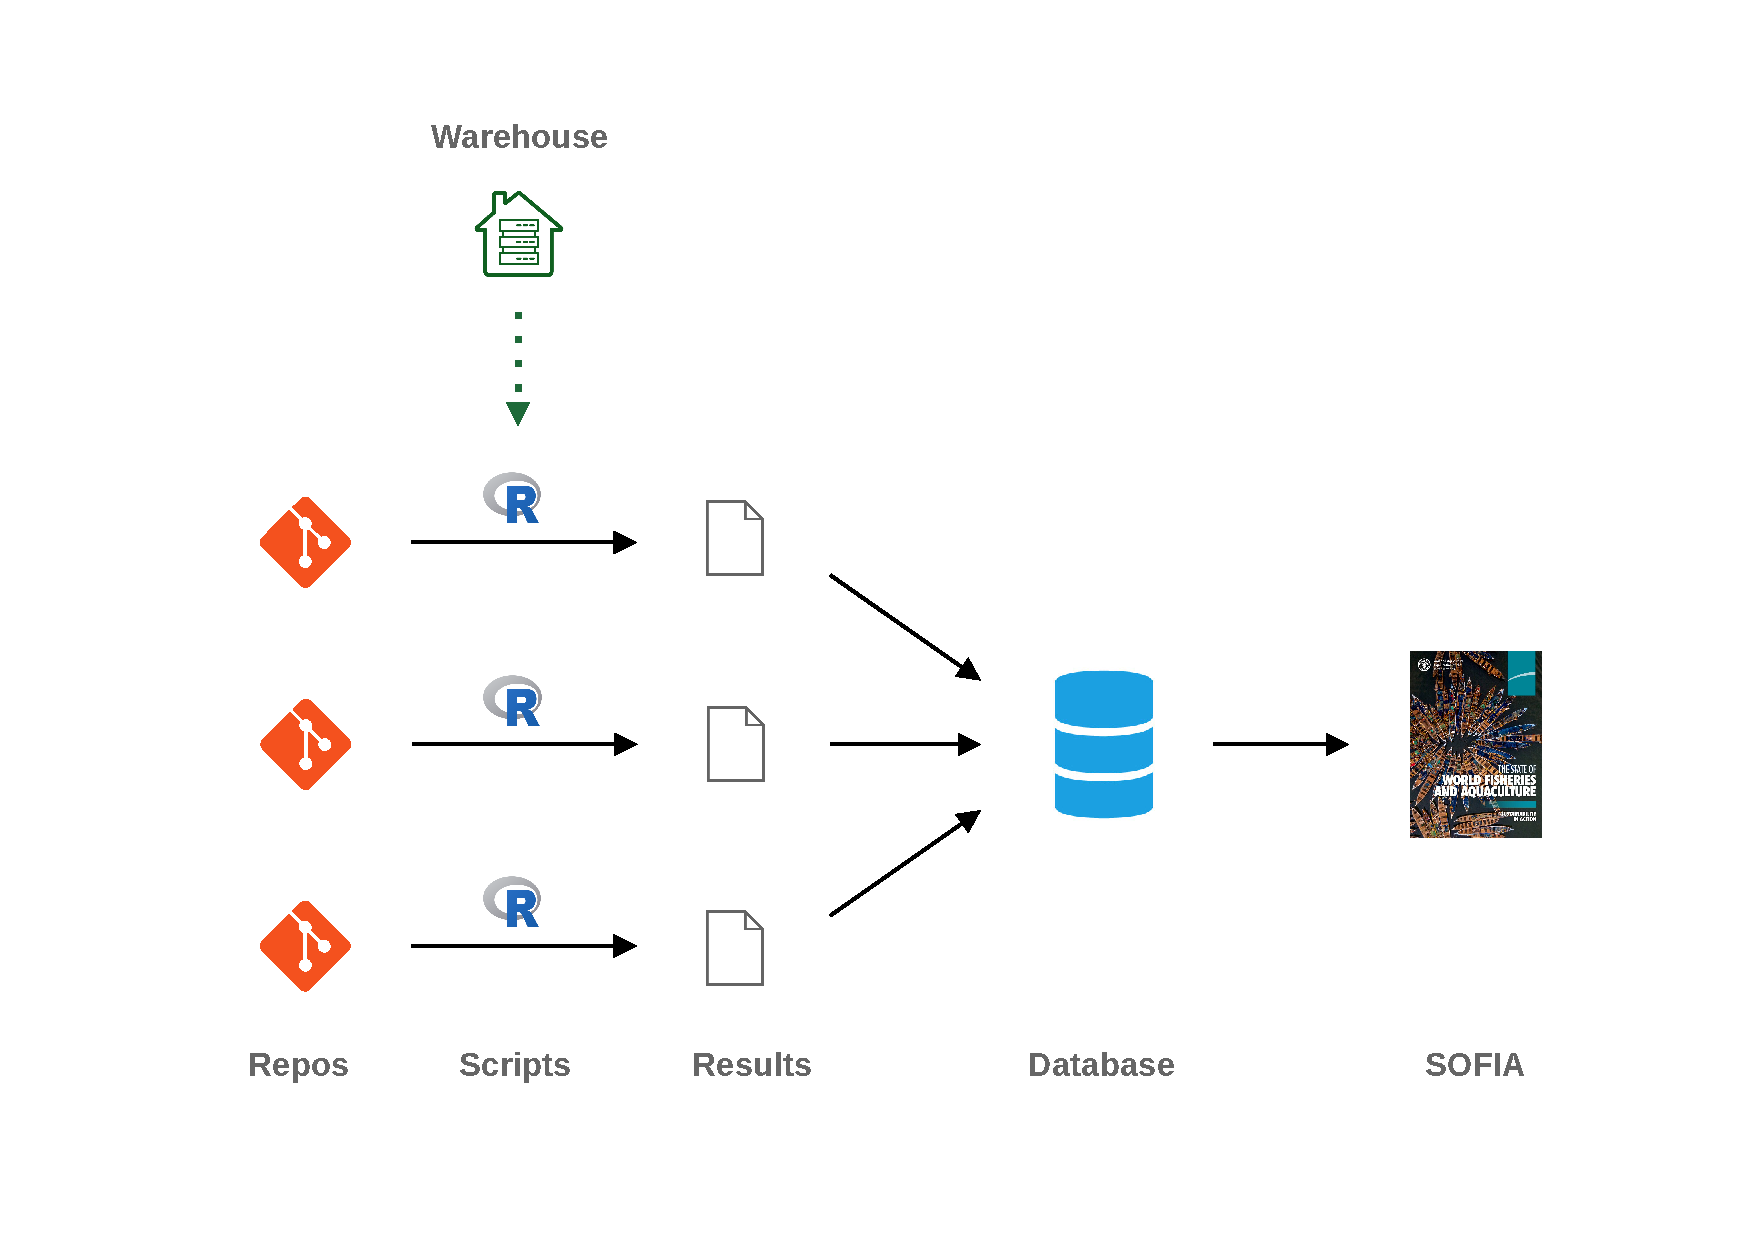
\includegraphics[width=0.8\textwidth]{sofia_taf_diagram}
    \vspace{2ex}
    \caption{SOFIA-TAF diagram, showing the flow of information from individual
      repositories (analyses of stocks and areas) to the final SOFIA report.}
    \label{fig:sofia-taf-diagram}
  \end{center}
\end{figure}

The scripts use a dedicated R package called \SOFIA. The next sections describe
each component of the SOFIA-TAF design in some detail: repositories, input data
warehouse, R package, and the database.

\subsection{SOFIA-TAF repositories}

\subsubsection{Repository features}

Each SOFIA-TAF repository is a unit of analysis, corresponding to a specific
area and a set of stocks. A GitHub repository, sometimes abbreviated as `repo',
is an online directory that is especially convenient for organizing text files,
such as scripts and data files. GitHub repository features relevant for
SOFIA-TAF include:

\begin{itemize}
  \item Ability to make scripts available online, for browsing and downloading,
  along with the input data required for the scripts to run.
  \item Automatic backup of all files with the ability to return to previous
  saved states.
  \item Tracked changes showing who changed what and when, supporting online
  teamwork.
  \item Ability to tag specific saved states of the analysis and give them
  descriptive names, such as `starting point`, `2021 data` or `results imported
  to database`.
  \item Ability to upload large attachments (\gt 100 MB) to accompany tagged
  states.
  \item Online facilities to compare text files and view changes, line by line.
\end{itemize}

\subsubsection{R scripts}

The analysis inside each repository consists of a set of R scripts that are
organized in TAF format (Magnusson and Millar 2021). This means there are four
standard scripts
(Table~\ref{tab:taf-scripts}) that conduct and document the analysis:\\[-1ex]

\begin{table}[htb]\small
  \caption{Standard TAF scripts for a given analysis.}
  \centering
  \begin{tabular}{ll}
    \hline
    Script          & Purpose\I{2.4ex}                                 \\
    \hline
    \verb|data.R|   & Preprocess data, write TAF data tables\I{2.6ex}  \\[0.6ex]
    \verb|model.R|  & Run analysis, write model results                \\[0.6ex]
    \verb|output.R| & Extract
                      results of interest, write TAF output tables     \\[0.6ex]
    \verb|report.R| & Prepare plots and formatted tables               \\[0.4ex]
    \hline
  \end{tabular}
  \label{tab:taf-scripts}
  \vspace{1.5ex}
\end{table}

The TAF scripts are run sequentially, each reading files that were created in a
previous step. The first script, \verb|data.R|, reads data files that were
declared and documented in a \verb|DATA.bib| text file. A similar
\verb|SOFTWARE.bib| file can be used to declare specific versions of software
used in the analysis, to strengthen reproducibility.

\begin{figure}[htb]
  \begin{center}
    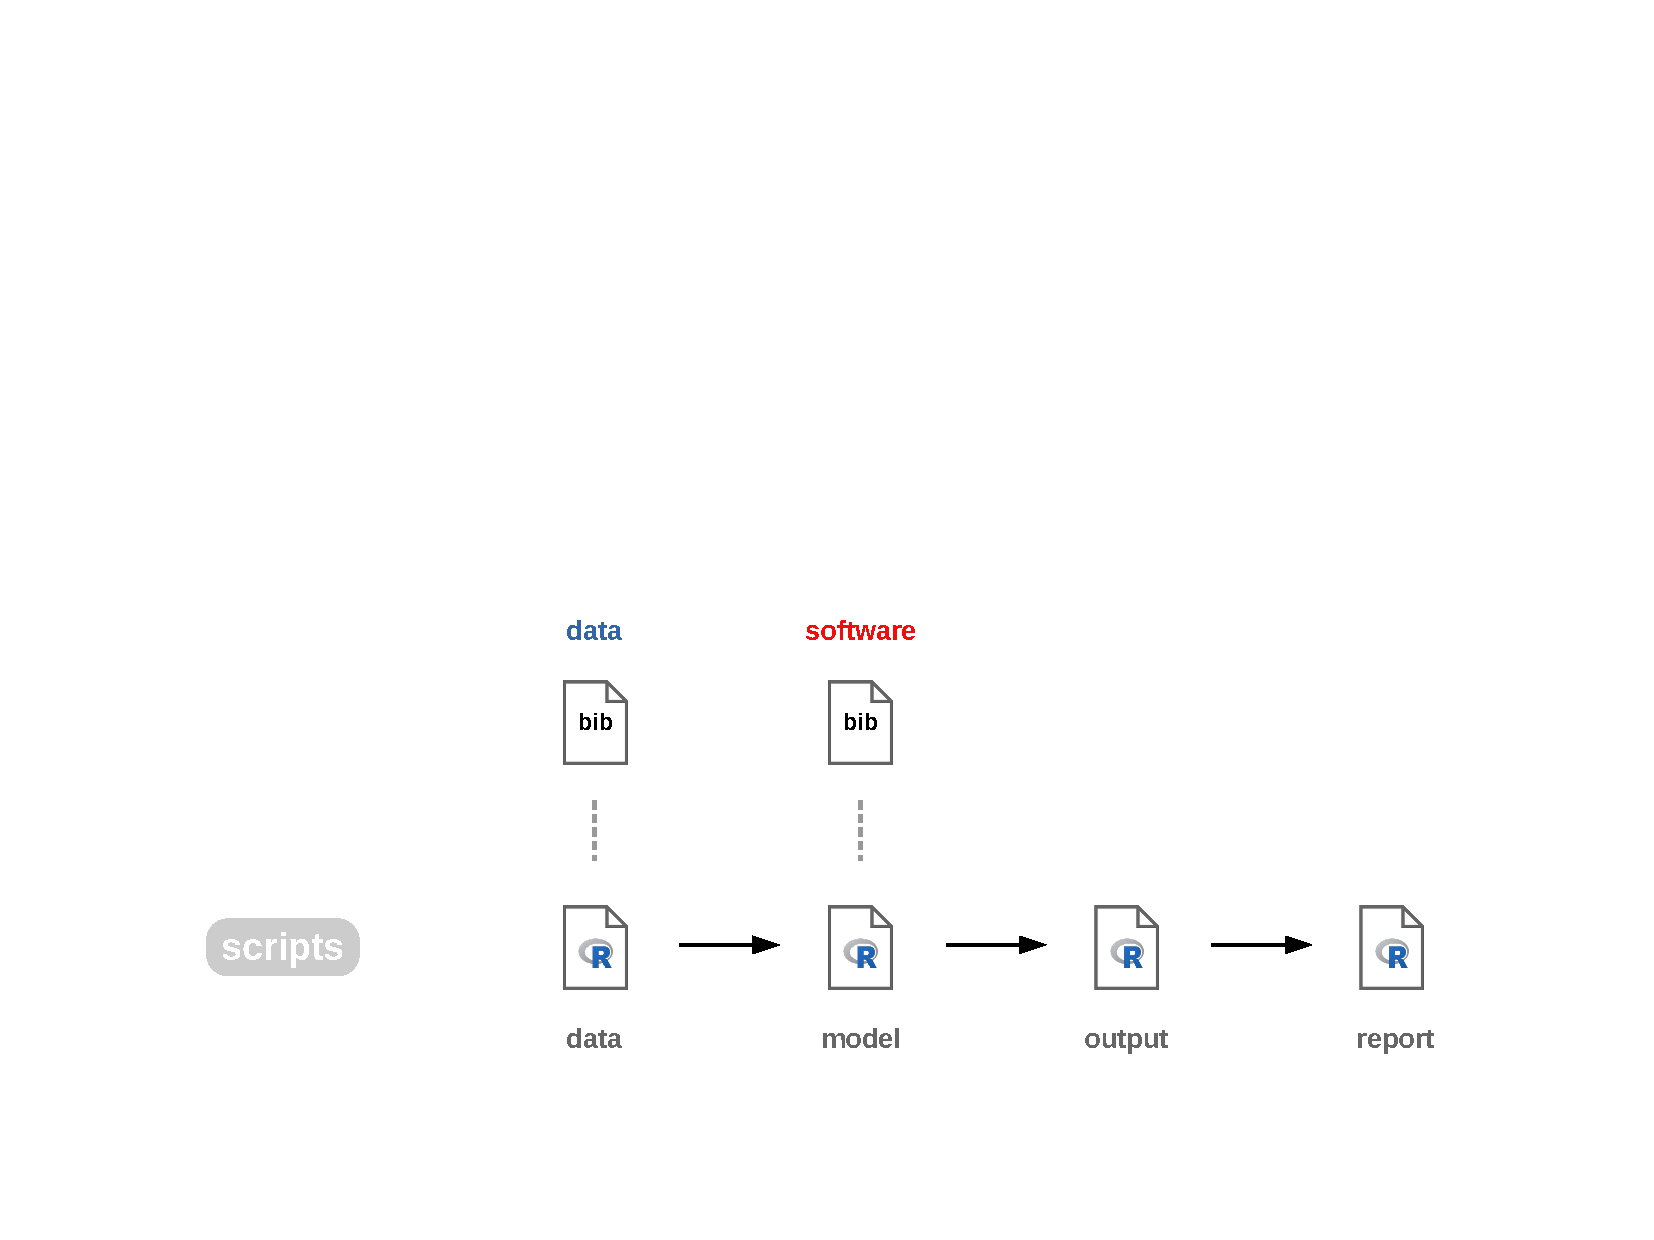
\includegraphics[width=0.8\textwidth]{taf_diagram}
    \vspace{2ex}
    \caption{TAF scripted workflow. Each SOFIA-TAF repository/analysis contains
      four standard R~scripts that are run sequentially. The initial data and
      software are declared in so-called bib files.}
    \label{fig:taf-diagram}
  \end{center}
\end{figure}

\newpage

The R scripts conducting SOFIA-TAF analyses rely especially on three R
packages:\\[-2ex]

\begin{itemize}
  \item \SOFIA\ -- a dedicated package to support SOFIA-TAF\\
  (Sharma and Magnusson 2022)
  \item {\sf TAF} -- utilities to manage scripts, data files, metadata, and R
  data objects\\
  (Magnusson and Millar 2021)
  \item {\sf sraplus} -- biomass dynamics model with Bayesian priors\\
  (Ovando 2022)
\end{itemize}

\subsubsection{Repository names and directory structure}

GitHub repositories are given descriptive names, such as

\qquad\blue{\url{https://github.com/sofia-taf/2021Area37Coastal}}

for the analysis conducted in 2021 of coastal stocks in Area 37.

On a personal laptop or a high-performance cluster, the SOFIA-TAF repositories
are organized in a hierarchical directory structure (Figure
\ref{fig:sofia-taf-dirs}), similar to the repository name as year/area/stock
group.\\

\begin{figure}[htb]
  \begin{center}
    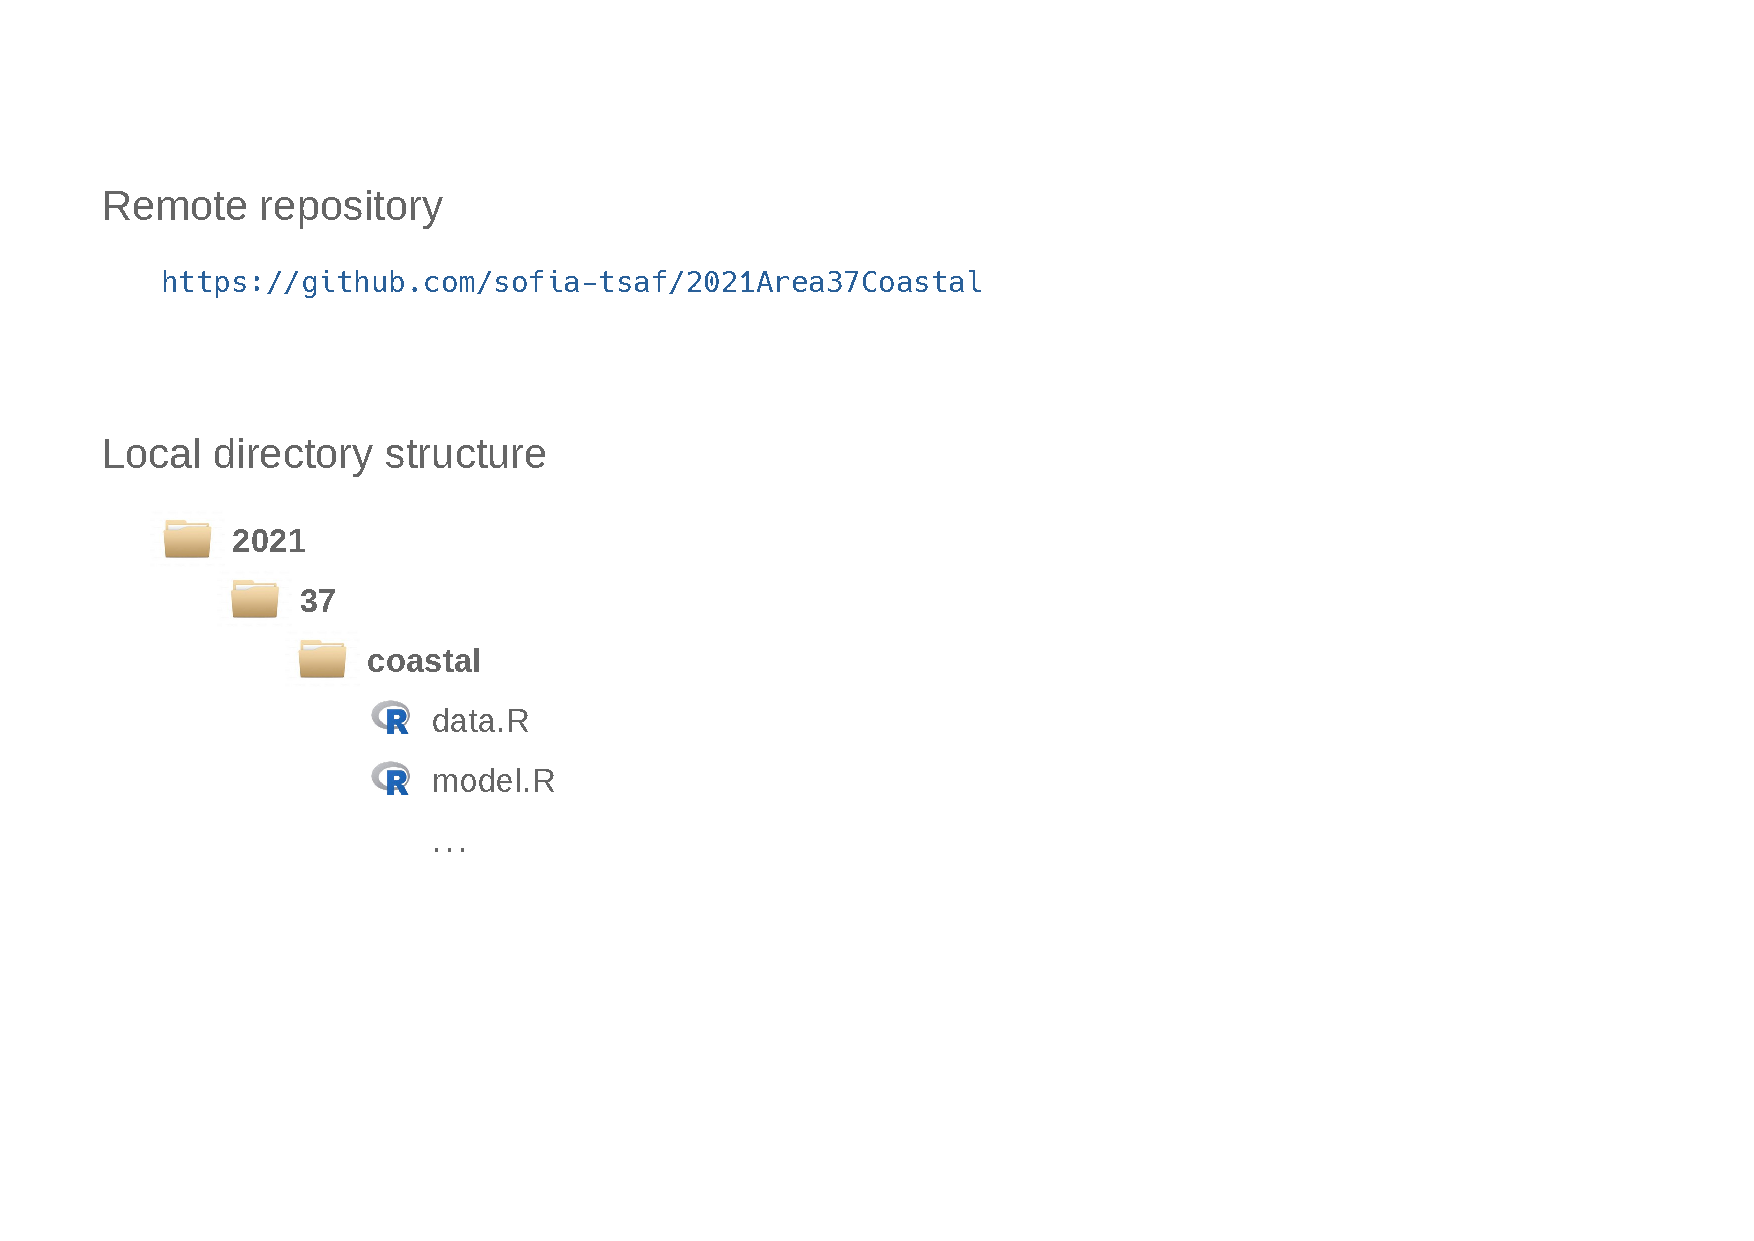
\includegraphics[width=0.6\textwidth]{sofia_taf_dirs}
    \vspace{1ex}
    \caption{SOFIA-TAF local directory structure, showing the similarity between
      the remote repository name and the local directory names.}
    \label{fig:sofia-taf-dirs}
  \end{center}
\end{figure}

\vspace{1ex}

This hierarchical directory structure is practical to navigate and run the
analyses, access results, and run top-level summary calculations across a large
number of analyses.

\subsection{Data collection templates}

SOFIA-TAF input data are collected and prepared in a collaborative process
between FAO and regional experts. The data used within a Tier 2 analysis are
organized in files such as {\tt catch.csv}, {\tt effort.csv}, and {\tt
  index.csv}, containing multiple stocks in each file. Data provided by regional
experts, however, are termed {\it primary} data files and are organized as one
file per stock, using filenames such as \verb|Yellowtail_snapper_Mexico.csv|.
The conversion from primary data files to Tier2 input data files is handled by
the \SOFIA\ package.

\subsection{Input data warehouse}

The input data warehouse contains fisheries data for all areas and stocks. Catch
and effort data for Tier 2 stocks are organized in two GitHub repositories:

\qquad\blue{\url{https://github.com/sofia-taf/catches}}

\qquad\blue{\url{https://github.com/sofia-taf/effort}}

Individual SOFIA-TAF analyses start by reading catch and effort data from the
data warehouse. In this way, the input data for all analyses are stored in one
central place, where they can be updated, documented, and quality checked.

\subsection{R package}

The \SOFIA\ package (Sharma and Magnusson 2022) contains utilities that are
commonly used in SOFIA-TAF analyses. It is developed in a dedicated GitHub
repository:

\qquad\blue{\url{https://github.com/sofia-taf/SOFIA}}

The \SOFIA\ package provides a single place to modify a large number of
SOFIA-TAF analyses. Incremental improvements become more manageable, e.g.,
changing the format of a specific plot, without having to edit each and every
SOFIA-TAF analysis. It also makes the R scripts for each analysis shorter and
thus easier to read, write, and maintain.

\subsection{Database}

The SOFIA-TAF database will contain the results from all the individual
SOFIA-TAF analyses. The primary focus of the database is on stock status, both
in numerical terms and in categorical terms: underfished, fully fished, and
overfished.

The database is the central node and key component of the SOFIA-TAF design. The
only way to enter data into the database is via SOFIA-TAF analyses, as indicated
in the SOFIA-TAF diagram (Figure \ref{fig:sofia-taf-diagram}), and when
SOFIA-TAF analyses of a specific areas and stocks are updated, the database is
automatically updated. Furthermore, the top-level analysis for the final SOFIA
report, aggregating a large number of SOFIA-TAF analyses, should be based on
queries to the database.

The above design guarantees the traceability of SOFIA results, all the way from
the individual datasets and analyses to the final published report.

The database is also a convenient stage in the pipeline to apply quality
control. Examples of quality checks could include referential integrity of
species and stock names, summary statistics at different levels of aggregation,
counting stocks in each area, plotting the distribution of numerical stock
status, etc. This will ensure that all stocks are accounted for, and reveal any
inconsistencies or issues that should be checked in the underlying analyses.

\newpage

% ______________________________________________________________________________

\section{Development status and next steps}

\subsection{SOFIA-TAF repositories}

\subsubsection{Current status}

As of end of December 2022, the GitHub site
\blue{\url{https://github.com/sofia-taf}} contains 32 SOFIA-TAF repositories, 12
that were created in 2021, and 20 created in 2022 (Table
\ref{tab:repository-count}).

\begin{table}[htb]\small
  \caption{Overview of SOFIA-TAF repositories.}
  \centering
  \begin{tabular}{llrl}
    \hline
    ~ & ~ & Number of\I{2.4ex}\\
    Year & Area & analyses & Specifically\\
    \hline
    2021 & Area 31   &  1 & Test\I{2.4ex}\\[0.2ex]
    ~    & Area 37   & 11 & ClamsOK, Coastal, Cods, Demersal, Flounder,\\
    ~    & ~         &  ~ & Herring, Other, Shads, Shimps, Squid, Test\\[0.5ex]
    2022 & Area 31   & 10 & CatchEffortGlobalv2JM, CatchOnly,\\
    ~    & ~         &  ~ & DemoEffortByStock, DemoEffortShared,\\
    ~    & ~         &  ~ & DemoIndexByStock, EffortJMstcks,\\
    ~    & ~         &  ~ & effortlocalcatchlocalv2JM, IndexMethodv2JM,\\
    ~    & ~         &  ~ & Indexstocks, Testnewstocks\\[0.2ex]
    ~    & Area 37   &  2 & Clams, Demo\\[0.2ex]
    ~    & Area 41   &  3 & DemoPriorsByStock, RelevantStocks\\[0.2ex]
    ~    & Area 57   &  4 & Efforttest, EffortTestNoPriornew70yrstocks,\\
    ~    & ~         &  ~ & Tier2FAOMonitored31withdepPrior,\\
    ~    & ~         &  ~ & Tier2FAOMonitorednodepPrior\\[0.2ex]
    ~    & Deep Seas &  1 & CCAMLR\\[0.1ex]
    \hline
  \end{tabular}
  \label{tab:repository-count}
  \vspace{1.5ex}
\end{table}

The status of all of these analyses is exploratory for development purposes, as
opposed to production analyses for a final SOFIA report. As development
progresses, some of the early exploratory repositories are left behind and will
only run with older versions of the \SOFIA\ package. Repositories under current
development have been updated to the current SOFIA-TAF version 2 format.

Five demo repositories were developed for regional SOFIA-TAF workshops that were
held in 2022:

\begin{itemize}
  \item \sofialink{2022Area37Demo}{2022Area37Demo}
  \item \sofialink{2022Area31DemoEffortShared}{2022Area31DemoEffortShared}
  \item \sofialink{2022Area31DemoEffortByStock}{2022Area31DemoEffortByStock}
  \item \sofialink{2022Area31DemoIndexByStock}{2022Area31DemoIndexByStock}
  \item \sofialink{2022Area37DemoPriorsByStock}{2022Area37DemoPriorsByStock}
\end{itemize}

\newpage

These five demos serve as a reference for SOFIA-TAF, demonstrating standardized
scripts for analyzing various combinations of effort data, survey index data,
and priors. As reference analyses, they will be updated and synchronized when
changes and improvements are introduced in the \SOFIA\ package and other
components of the SOFIA-TAF framework.

To strengthen the reproducibility aspect of running SOFIA-TAF, analyses created
in 2022 have used the \verb|SOFTWARE.bib| file to declare the version of the
\SOFIA\ package that is required to run a given analysis. This has been
especially useful after the release of version 2 of the \SOFIA\ package in
August 2022.

Near the end of 2022, a new GitHub site
\blue{\url{https://github.com/sofia-taf-dev}} was created, as an alternative
place from \blue{\url{https://github.com/sofia-taf}} to organize development.
One approach to manage SOFIA-TAF would be store experimental analyses on the
`dev' site and production analyses on the main site.

\subsubsection{Next steps}
\label{subsubsec:repos-next-steps}

\textbf{Read from input data warehouse}

Currently, the SOFIA-TAF analyses read catch and effort data from a local data
directory, specific to each analysis. This means that data are repeated between
analyses, especially the effort data. Furthermore, to update catch and effort
data, one would have to modify a large number of SOFIA-TAF repositories. The
input data warehouse offers a more efficient, traceable, and quality-controlled
workflow.\\[-2ex]

\textbf{Categorical status by stock and year}

SOFIA-TAF analyses produce an output file called \verb|stock_timeseries.csv|
with numerical $B/B_\mathrm{MSY}$ and $F/F_\mathrm{MSY}$ by stock and year. For
the subsequent analysis, it would be beneficial if the categorical stock status
(underfished, fully fished, overfished) by year is also included in this file.
This improvement will require
modifications to the \verb|output.R| script of all SOFIA-TAF analyses.\\[-2ex]

\textbf{Managing repositories}

During the development of SOFIA-TAF, a number of experimental analyses have been
created as repositories on the main \blue{\url{https://github.com/sofia-taf}}
site. Some analyses can be considered will become production analyses for a
final SOFIA report, whose results should be imported into the SOFIA-TAF
database, while other analyses should probably be migrated to the development
area on \mbox{\blue{\url{https://github.com/sofia-taf-dev}}}. Some older
experimental analyses could be deleted, if they have been superseded by more
recent analyses.\\[-2ex]

When importing results from analyses into the SOFIA-TAF database, the relevant
analyses could be defined as all repositories on
\blue{\url{https://github.com/sofia-taf}} whose name begins with year and area.

\newpage

\textbf{Managing output files}

A significant challenge in SOFIA-TAF is that each analysis takes considerable
time to run (\gt 1 hr) and produces large output files (\gt 100 MB). Every time
a small update is made to the scripts or underlying data, a new run is required
and the output files are likely to change. SOFIA-TAF development so far has
explored two approaches to store the output files.

Approach 1. Initial development (e.g., \verb|area37|) kept the output files
outside of the repository. Instead of uploading the output files along with the
R scripts, output files were uploaded as GitHub `release assets'. The advantage
of this approach is that the repository remains very light and easy to work
with, and takes much less space on the hard drive of a personal laptop.

Approach 2. Later development (e.g., \verb|2021Area37Coastal|) has the output
files stored inside the repository. The advantage of this approach is that it
reduces the need to manage tags and GitHub releases, and makes it slightly less
likely to have mismatching R scripts and output files.

Unfortunately, neither of the above approaches can guarantee a correct match
between the R scripts and the output files. In other words, when a change is
made to an R script and uploaded to the repository, it's easy to forget or omit
running the entire analysis and uploading new output files.

A 3rd approach worth exploring would be not to upload output files to the GitHub
repository at all. Instead, the database server would run all analyses locally.
Specifically, a GitHub webhook could be developed, so that whenever a change is
uploaded to the GitHub repository, the database server pulls the changes, runs
the analysis and imports the results into the database. This would guarantee a
strong linkage between the SOFIA-TAF repositories and the database.\\[-2ex]

\subsection{Data collection templates}

\subsubsection{Current status}

The data collection templates are under development. For Tier 2, a prototype of
the conversion process from primary data files (provided by regional experts) to
SOFIA-TAF format has been implemented in the \SOFIA\ package, where {\tt
  groupData} organizes primary data files into subdirectories and {\tt
  convertData} converts them to SOFIA-TAF format.

The Tier 2 prototype functions {\tt groupData} and {\tt convertData}
perform quality control and raise descriptive error messages if a primary data
file does not meet the criteria required for data conversion to SOFIA-TAF
format.

\subsubsection{Next steps}

Data collection templates for Tiers 1, 2, and 3 will be further developed in
2023. For Tier 2, the primary data files should be in a format that meets the
criteria of the {\tt groupData} and {\tt convertData} functions.

\subsection{Input data warehouse}

\subsubsection{Current status}

The \blue{\url{https://github.com/sofia-taf/catches}} repository currently
contains the following file with catch data:

\begin{verbatim}
cap_2021-10-17_193245.csv
\end{verbatim}

The \blue{\url{https://github.com/sofia-taf/effort}} repository has been created
but is still empty.

\subsubsection{Next steps}

The data in the \verb|catches| repository data are ready for exploratory use,
testing the ability of R scripts to read catch data from the central warehouse
instead of a local data directory.

Data can be added to the \verb|effort| repository in CSV format. Alternative
structures of the data will be evaluated, before deciding how to organize the
effort data from different areas and stocks.

For SOFIA-TAF analyses of Tier 1 and 3, the data warehouse can incorporate the
underlying numerical and categorical data from official stock assessments and
expert elicitation. This could further increase the clarity and traceability of
the overall SOFIA analysis of stock status.

\subsection{R package}

\subsubsection{Current status}

Version 2.1.1 of the \SOFIA\ package was released on 15 Nov 2022. The package
help page that comes with \SOFIA\ lists the following functions, categorized by
functionality.\\[-2ex]

{\it Prepare data:}

\begin{tabular}{ll}
  {\tt addDriors}   & add driors column to stocks object\\
  {\tt addEffort}   & add effort column to catch data\\
  {\tt addIndex}    & add index column to catch data\\
  {\tt convertData} & convert primary data to combined data\\
  {\tt groupData}   & group primary data in subdirectories\\[1.5ex]
\end{tabular}

\newpage

{\it Calculate:}

\begin{tabular}{ll}
  {\tt calcCat} & stock status categories\\[1.5ex]
\end{tabular}

{\it Plot:}

\begin{tabular}{ll}
  {\tt plotCat} & summary of stock status categories\\[1.5ex]
\end{tabular}

{\it Repositories:}

\begin{tabular}{ll}
  {\tt gitRepos}    & list GitHub repositories\\
  {\tt gitClone}    & clone GitHub repository\\
  {\tt gitCloneAll} & clone all SOFIA-TAF repositories\\[1.5ex]
\end{tabular}

The current status of the package is stable and fully documented, passing a
strict \verb|R CMD --as-cran| quality check. Table \ref{tab:package-history}
shows the complete release history.

\begin{table}[htb]\small
  \caption{\SOFIA\ package release history.}
  \centering
  \begin{tabular}{lrl}
    \hline
    Version & Date & New functions\\
    \hline
    2.1.1   & 2022-11-15 & ~\I{2.3ex}\\[0.8ex]
    2.1.0   & 2022-11-11 & {\tt addIndex}\\[0.8ex]
    2.0.0   & 2022-08-08 & {\tt gitRepos}, {\tt gitClone}, {\tt
                           gitCloneAll}\\[0.8ex]
    1.2.1   & 2022-05-21 & ~\\[0.8ex]
    1.2.0   & 2022-02-25 & {\tt convertData}\\[0.8ex]
    1.1.0   & 2022-02-20 & {\tt groupData}\\[0.8ex]
    1.0.3   & 2022-02-14 & ~\\[0.8ex]
    1.0.2   & 2022-01-24 & {\tt addDriors}, {\tt addEffort}, {\tt calcCat},
                           {\tt plotCat}\I{2.3ex}\\
    \hline
  \end{tabular}
  \label{tab:package-history}
  \vspace{1.5ex}
\end{table}

A more detailed list of changes introduced in each version of the \SOFIA\
package can be found online at
\blue{\url{https://github.com/sofia-taf/SOFIA/blob/main/NEWS.md}}.

\subsubsection{Next steps}

One area of the \SOFIA\ package that can be developed is the creation of QC
functions to apply quality control for SOFIA-TAF analyses, identifying possible
mistakes in the analyses that can then be fixed.

\newpage

\subsection{Database}

\subsubsection{Current status}

The database of SOFIA results is implemented in MySQL. Its development is
organized in a GitHub repository:

\qquad\blue{\url{https://github.com/sofia-taf/database}}

Database import and export is managed using Bash shell scripts, which are found
in the GitHub repository.

\subsubsection{Next steps}

\textbf{Strong link between repositories and database}

The link between SOFIA-TAF repositories and the database of results (Figure
\ref{fig:sofia-taf-diagram}) is essential for traceability and the fundamental
purpose of SOFIA-TAF. The very basis of the SOFIA-TAF design is that the results
found in the database should match exactly the results produced by the SOFIA-TAF
repositories.

One database script under development loops through the list of repositories and
pulls down the \verb|current_status.csv| file to ingest to the database.

The design and development of this linkage is still ongoing, including automatic
detection of which analyses contain results that should be imported into the
database. The separation of repositories into production analyses on
\blue{\href{https://github.com/sofia-taf}{\sf sofia-taf}} and experimental
analyses on \blue{\href{https://github.com/sofia-taf-dev}{\sf sofia-taf-dev}}
(Section \ref{subsubsec:repos-next-steps} on `Managing repositories') is related
to designing a strong link between repositories and the database of SOFIA-TAF
results.\\[-2ex]

\textbf{Database server managing SOFIA-TAF output files}

One design possibility is to have a dedicated SOFIA-TAF database server as the
main platform to run SOFIA-TAF analyses and manage output files, in addition to
importing the results into the database.

The development goal `Managing output files' (Section
\ref{subsubsec:repos-next-steps}) elaborates on this possible approach, which
could involve a GitHub webhook to establish a reliable pipeline of information
from SOFIA-TAF repositories to the database.

\newpage

\section{Acknowledgements}

Working with Rishi Sharma and Nicole Tursich on this project is a privilege and
joy. Our domains of expertise complement each other, and we share a common
vision and enthusiasm to enhance the FAO infrastructure and analytical workflows
for estimating the state of the world's fisheries. I would like to acknowledge
Colin Millar for our collaboration in creating TAF (Magnusson and Millar 2021),
which has served as an inspiration and basis for the SOFIA-TAF design. Last but
not least, I~am grateful to Pedro Barros and colleagues at FAO for their
guidance and vote of confidence for this technical development project.

\vspace{3ex}

\section{References}

\small\sloppy\setlength\hyphenpenalty{1000}\selectfont
\begin{description}\setlength\itemsep{0.5ex}\vspace{0.5ex}

  \item FAO (Food and Agriculture Organization of the United Nations). 2020. The
  State of World Fisheries and Aquaculture 2020: Sustainability in action. Rome.
  206 pp.\\
  \blue{\footnotesize\url{https://doi.org/10.4060/ca9229en}}

  \item Magnusson, A. 2021. SOFIA Transparent Analytical Framework: Design and
  development progress.\\
  \blue{%
    \footnotesize\url{https://arni-magnusson.github.io/pdf/2021-sofia-taf.pdf}}

  \item Magnusson, A. and C. Millar. 2021. TAF: Functions to Support the ICES
  Transparent Assessment Framework. R package version 4.0.0.\\
  \blue{\footnotesize\url{https://cran.r-project.org/package=TAF}}

  \item Ovando, D. 2022. sraplus: Run sraplus Assessments. R package version
  3.7.5.\\
  \blue{\footnotesize\url{https://github.com/DanOvando/sraplus}}

  \item Sharma, R. and A. Magnusson. 2022. SOFIA: Tools to Work with SOFIA-TAF
  Analyses. R package version 2.1.1.\\
  \blue{\footnotesize\url{https://github.com/sofia-taf/SOFIA}}

\end{description}

\normalsize

\newpage

\appendix

\section{Arni's contributions in 2022}

\textbf{SOFIA-TAF design}

The work on this project is divided been design and development. The design part
takes place largely during online technical meetings of the SOFIA-TAF
development team, and is the product of dynamic teamwork and discussions. As the
SOFIA-TAF design borrows both ideas and technical components from TAF (Magnusson
and Millar 2021), Arni has served in a lead role in the design of many aspects
of SOFIA-TAF, especially the structure of SOFIA-TAF repositories, input data
warehouse, and the
R~package.\\[-2ex]

\textbf{SOFIA-TAF repository development}

On the development front, Arni has created and updated five demo repositories
that serve as serve as a reference, demonstrating the current and
recommended format for SOFIA-TAF analyses.\\[-2ex]

\textbf{Teaching and documenting}

For the regional workshops in 2022, Arni gave presentations and participated in
discussions to explain the overall design of SOFIA-TAF and how data files and R
scripts perform the analysis of stock status. The goal is to enable regional
experts to contribute the best data available to SOFIA-TAF.

For the SOFIA-TAF launch event at the CAPAM conference, Arni gave a presentation
describing the importance of open and reproducible analyses in fisheries
science, and how the SOFIA-TAF design is centered on those objectives.

All functions of the \SOFIA\ package are fully documented and updated with each
release. Arni has also analyzed the extent of package dependencies of the {\sf
  sraplus} package, which is especially relevant for the reproducibility aspect
of SOFIA-TAF analyses.\\[-2ex]

\textbf{R package}

Arni maintains the \SOFIA\ package, acting as a single place of analytical
methods used in all SOFIA-TAF analyses. This greatly improves the ability to
manage and maintain the large number of SOFIA-TAF analyses behind SOFIA.\\[-2ex]

\textbf{Contributions to project management}

With this report, updated annually, Arni has aimed to describe the current
status and next steps in the development of SOFIA-TAF, especially the aspects
relating to the analyses (data, scripts, and results) and the underlying \SOFIA\
package. This conveys a design manifesto and has helped to track progress, set
objectives, and provide an up-to-date documentation of how the SOFIA-TAF
components work together.

\newpage

\textbf{Links to deliverables}

\begin{itemize}
  \item[-] Demo analyses:\\[-3.5ex]
  \begin{itemize}
    \item[] \sofialink{2022Area37Demo}{2022Area37Demo}\\[-4ex]
    \item[] \sofialink{2022Area31DemoEffortShared}
    {2022Area31DemoEffortShared}\\[-4ex]
    \item[] \sofialink{2022Area31DemoEffortByStock}
    {2022Area31DemoEffortByStock}\\[-4ex]
    \item[] \sofialink{2022Area31DemoIndexByStock}
    {2022Area31DemoIndexByStock}\\[-4ex]
    \item[] \sofialink{2022Area37DemoPriorsByStock}
    {2022Area37DemoPriorsByStock}\\[-3ex]
  \end{itemize}
  \item[-] Presentations:\\[-3.5ex]
  \begin{itemize}
    \item[] Area 31
    (\sofialink{doc/blob/main/presentations/area_31/overview.pdf}{overview},
    \sofialink{doc/blob/main/presentations/area_31/demo.pdf}{demo})\\[-4ex]
    \item[] Area 41
    (\sofialink{doc/blob/main/presentations/area_41/overview.pdf}{overview},
    \sofialink{doc/blob/main/presentations/area_41/demo.pdf}{demo})\\[-4ex]
    \item[] \sofialink{doc/blob/main/presentations/capam/open_reproducible.pdf}
    {CAPAM} conference\\[-3ex]
  \end{itemize}
  \item[-] \sofialink{doc}{Documentation} page, including sraplus
  \sofialink{doc/blob/main/sraplus_dependencies.md}{dependencies} and
  \sofialink{doc/blob/main/sraplus_history.md}{history}\\[-3ex]
  \item[-] \sofialink{SOFIA}{SOFIA} package\\[-3ex]
  \item[-] \blue{\href{https://arni-magnusson.github.io/pdf/2022-sofia-taf.pdf}
    {{\sf This}}} current report
\end{itemize}

\end{document}
